\documentclass[12pt]{article}

\usepackage{fullpage}
\usepackage{multicol,multirow}
\usepackage{tabularx}
\usepackage{ulem}
\usepackage[utf8]{inputenc}
\usepackage[russian]{babel}
\usepackage{graphicx}
\usepackage{indentfirst}


\begin{document}

\section*{Лабораторная работа №\,8 по курсу дискрeтного анализа: Жадные алгоритмы}

Выполнил студент группы М8О-207Б МАИ \textit{Цапков Александр}.

\subsection*{Условие}

\begin{enumerate}
\item Разработать жадный алгоритм решения задачи, определяемой своим вариантом. Доказать его корректность, оценить скорость и объём затрачиваемой оперативной памяти.

Реализовать программу на языке С или С++, соответсвующую построенному алгоритму. Формат входных и выходных данных описан в варианте задания.
\item Вариант: 4

Бычкам дают пищевые добавки, чтобы ускорить их рост. Каждая добавка содержит некоторые из N действующих веществ. Соотношенияколичеств веществ в добавках могут отличаться. Воздействие добавки определяется как $c_1 a_1 + c_2 a_2 +...+c_N a_N$, где $a_i$ количество i-го вещества в добавке, $c_i$ — неизвестный коэффициент, связанный с веществом и не зависящий от добавки. Чтобы найти неизвестные коэффициенты $c_i$, Биолог может измерить воздействие любой добавки, использовав один её мешок. Известна цена мешка каждой из $M (M >= N )$ различных добавок. Нужно помочь Биологу подобрать самый дешевый наобор добавок, позволяющий найти коэффициенты $c_i$. Возможно, соотношения веществ в добавках таковы, что определить коэффициенты нельзя.

\end{enumerate}

\subsection*{Метод решения}
Для начала приведем задачау к более математическому и формальному виду. Для нпхождения n коэффициентов $с$ нужно ровно n дабавой (n уравненией). Эти коэффициенты найдуться одназначно, когда матрица n*n из весов a будет иметь не нулевой детерминант (по теореме крамера). Тогда задачу сведем к: поиску системы линейно независимых строк с наименьшей суммарной стоимостью. Для этого мы возьмем все строки, отсортируем их по возрастанию цены и начнем добовлять их в итоговую матрицу. Если очереднaя строка является линейно-зависимой, то ее мы не добавлеям. Проверка на линейную зависимость идет по алгоритму Гауса. Таким образом если мы заполнили n строк, то мы нашли ответ, а если до конца m не заполнили все n строк, то решить систему невозможно.


\subsection*{Описание программы}

Моя программа состоит из 1 файла main.cpp. В нем имеется структура TLine, в которой зраниться информация о строке и перегруженные операторы для вычитания строк и умнажения их на число (а также сравнение по цене). В самой программе вы сначала считываем все строки в вектор и сортируем их по возрастанию. После этого начинаем заполнять вектор строк размера n (это и есть результирующая матрица). При заполнении мы добовляем строку на следующую позицию после последней добавленной. Затем вычитаем из нее предыдущие строки так, чтобы получился независимый остаток. Есди вся строка нулевая, значит она линейно зависимая и мы пытаемся добавить сл. строку. Если же мы находим ненулевой элемент, то мы нормируем строку разделяя ее на этот ненулевой элемент. Алгоритм заканчивается когда n строк заполнены или же когда кончаются m строк.
\subsection*{Дневник отладки}

1-я посылка: неправильный ответ. Забыл убрать отладочный принт.

2-я посылка: ошибка выполнения. выходил за пределы массива из-за ошибке в счетчике

3-я посылка: ожидает подтверждения.
\subsection*{Тест производительности}
При максимальном m зависимость времени выполнения от n линейна, так как на каждой итерации мы просто выполняем чуть больше действий (для каждой строки). Вносит неточность и случайные быстро нейденные решения при маленьктх n, так что я построил график по среднему времени за 100 проходов. Вот результат:
 
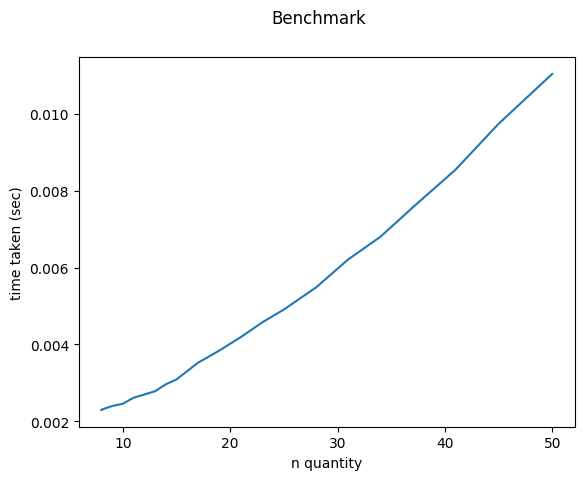
\includegraphics[width=440pt]{m.png}

На графике мы можем наблюдать небольшое искревление. Это связано скорее всего с тем что я использкю сортировку, которая работает не за линейное время.

\subsection*{Выводы}

В данной лабарвторной работе мне впервые понадобились знания матеманики(в частности линейной алгебры) в чистом виде. До этого я всегда пользовался алгоритмами ДА или же других предметов по программированию, но в этот раз решение задачи и ее понимание лежало именно на понимании линейной алгебры. Знание нужных теорем позволило куда быстрее придумать и реализовать решение. Доходить до алгоритма решения без них было бы куда сложнее.

\end{document}

